This section discusses the methods to identify the presence of hyper giants in today's Internet and to find out the inter dependency between hyper giants and popular websites. It is commonly known that most of the websites use some kind of hosting infrastructure for distributing their Internet content. This hosting infrastructures can be CDN, cloud computing infrastructure or content providers. Hosting infrastructures were designed to transport and cache large amounts of Internet content, such as HTML code, JavaScript, large files, images, audio, and video. The most appropriate way to identify whether a website is using a hosting infrastructure service is to inspect its HTML code looking for URLs linked to hosting infrastructure. The redirection of a link to an external hosting company will be clear evidence that a particular website is using a hosting infrastructure. 

To perform this task, as shown in figure, 100000 top ranked websites of Alexa will be crawled using scrapy engine and their HTML codes  are inspected to retrieve all their embedded URLs.Then these URLs will be used to find out the link redirection and subsequently the hosting infrastructure. DNS resolution is the known solution to find out the link redirection. It will resolve the web URL into single or multiple  IP addresses and their corresponding ARecord names. ARecord names show the hosting infrastructure linked to corresponding URL. Sometimes hosting companies use different naming convention to represent their ARecords. As an example, a1586.b.akamai.net. and a1586.a.akamai.net are the ARecord names when www.bmw.com is resolved. This might be because of load balancing the servers that are used to cache content. Therefore, to get the desired hosting infrastructure ,the second level domain (SLD) of each ARecord is the best suited option.

The set of IP addresses for a particular SLD shows the degree to which the corresponding hosting infrastructure is connected with different web URLs. The number of BGP prefixes show the network footprint and the number of ASNs show how the infrastructure is distributed. Therefore, to identify the hyper giants, the natural choice for the features to consider are IP addresses, AS Numbers and the BGP prefixes.

Hyper giants build a large infrastructure all around the world to deliver content ensuring a faster response. The websites use these infrastructure to store their content, such as audios ,videos, test/html files etc. Therefore, any kind of disruption in serving these contents from hyper giants will impact the websites which shows the interdependency of hyper giants with the web sites. To know which content type will be impacted more, the type of content can be studied. To evaluate the type of content,as shown in figure, HTTP header analysis will be carried out on 100000 top ranked websites of Alexa and their corresponding embedded URLs. The web object type retrieved from the HTTP header information determines the content type such as text/html, image, video, audio etc., which will be used to analyze the interdependency between hyper giants and these websites.

\begin{figure}[h]
\includegraphics[width=\textwidth,height=10cm]{/home/sakib/soumya/wholeSLD/method-1.png}
\centering
\caption{High level approach Part-1}
\end{figure}

\begin{figure}[h]
\includegraphics[width=\textwidth,height=10cm]{/home/sakib/soumya/wholeSLD/method-2.png}
\centering
\caption{High level approach Part-2}
\end{figure}

\subsection{Identification of hyper giants}
To find out the hyper giants in Internet,the hosting infrastructure which are serving popular websites will be observed. This can be determined by analyzing different features of hosting infrastructure such as IP addresses, BGP prefixes, ASN numbers etc. The methods to find out these features will be discussed in the following subsections.
\subsubsection{Hosting infrastructure to BGP Prefix Mapping}
\begin{figure}[h]
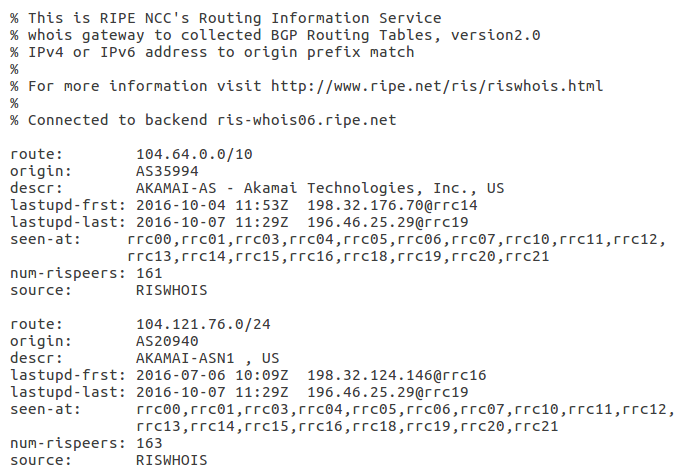
\includegraphics[width=\textwidth,height=10cm]{/home/sakib/soumya/latexNew/whois.png}
\centering
\caption{RIPE RIS bgp prefixes using whois command}
\end{figure}
From DNS resolution, the hosting infrastructure and corresponding IP addresses are determined. To find out BGP prefix routes of a particular IP address, BGP routing information from RIPE RIS [23] will be used. In figure-7, "route" shows the BGP prefixes of a IP address. From the figure this can be observed that the IP address 104.121.76.73 can be routed via two different prefixes 104.64.0.0/10 and 104.121.76.0/24. So both the prefixes for this IP will be considered for further analysis. This procedure will be carried out for each IP addresses of hosting infrastructure which will result in (hosting infrastructure, prefixes) mapping.

\subsection{Clustering}
From the initial analysis on the data collected for analyzing hosting infrastructure, it is found out that some hosting infrastructure are administered by the same company. For example, both the hosting infrastructure akamaiedge.net and akamai.net are administered by the same company, Akamai. Similarly google.com, googleusercontent.com, googlehosted.com and googledomains.com are administered by same company, Google. Generally companies use different ARecord names depending on the type of service they offer and the geographical location from where they offer the services. It is observed that Amazon uses two different ARecord names, namely amazonaws.us-east-1.elb.amazonaws.com, eu-west-1.elb.amazonaws.com for its customers from two geographical locations. It has to be analyzed, whether these ARecord names are pointing to same infrastructure or different. If they are pointing to the same infrastructure, they should be considered as one, else separately. This can be identified by using clustering algorithm by analyzing the BGP prefixes they share. 

The clustering algorithm takes a two step approach. In the first step, the prefixes of the hosting infrastructure will be aggregated into set of parent prefixes as explained in 3.2.1. In the subsequent step, the parent prefixes of the hosting infrastructure will be compared with each of the remaining infrastructure for clustering as explained in section 3.2.2.
\subsubsection{Prefix Aggregation of hosting infrastructure}
From the section 3.1.2, hosting infrastructure mapped to corresponding BGP prefixes are collected. But in this mapping, it is observed that some of the BGP prefixes are subset of other BGP prefixes. For example, googledomains.com has the prefix set ’216.239.32.0/19’, ’216.239.32.0/24’, ’216.239.34.0/24’, ’216.239.36.0/24’ and ’216.239.38.0/24’. Here the prefixes ’216.239.32.0/24’, ’216.239.34.0/24’, ’216.239.36.0/24’, ’216.239.38.0/24’ are subnet of prefix ’216.239.32.0/19’. Hence it is ideal to aggregate them. This way all the child prefixes in each mapping are aggregated to their parent prefixes. By end of this method, each hosting infrastructure will be mapped to a set of parent prefixes. For example, the hosting infrastructure googledomains.com is mapping to the parent prefix ’216.239.32.0/19’, as all child prefixes got aggregated into '216.239.32.0/19' parent prefix. This procedure is repeated for all the other infrastructure mappings, which generates a complete list of hosting infrastructure to their corresponding aggregated BGP prefixes.These mapping are sorted in the decreasing order of links hosting by each of these hosing infrastructure.The motivation behind doing this, is to allow the merging of smaller infrastructure into the larger one depending on their similarity factor (sim(s1, s2)) which is discussed in next section.

\subsubsection{Evaluation of Similarity between two hosting infrastructure}
The possibility of clustering any two hosting infrastructures is determined by analyzing the similarity between their aggregated prefixes. This can be done by verifying if one prefix is a parent to the other. While comparing two hosting infrastructures, if any of the hosting infrastructure contain child prefix of other, then the child prefix will be replaced with the parent prefix. This will make two prefix sets homogeneous, thus helping in evaluating the degree of the similarity between them. For comparing two hosting infrastructures, the similarity equation is defined as follows,

The similarity factor sim(s1,s2) is defined as follows,
\begin{equation}
sim(s1, s2)= \frac{|s1 \cap s2|}{|s2|}
\end{equation}

where s1,s2 are the bgp prefix sets.

If the similarity between two prefix sets are greater than equal to the 70\%, then both the hosting infrastructure will be clustered together making them a single clustered infrastructure. It is assumption that, s2 can be clustered with s2, provided 70\% of s2's prefixes are from that of s1's. This procedure will be repeated for all the hosting infrastructure. If two infrastructure has similarity factor greater than equal to 0.7, then the child hosting infrastructure will be merged into the parent hosting infrastructure and will be excluded from further comparisons. For example ’googleusercontent.com’ matched with ’google.com’ with similarity factor 1. This does not mean that both these hosting infrastructure has the same set of prefixes, but it means that, ’googleusercontent.com’ shares 100\% of its prefixes with ’google.com’. Once this is matched, ’googleusercontent.com’ will not be available for any further similarity matching with any other hosting infrastructures. It is assumed that a similarity index of grater than equal to 0.7 served as a good measure to determine the degree of similarity between two hosting infrastructure which can be considered as future work for extensive analysis.A sample example is explained as follows,

\begin{center}
\fbox{\begin{varwidth}{\dimexpr\textwidth-2\fboxsep-2\fboxrule\relax}

Let (hosting infrastructure,Prefix set)s are,
(SLD1,[10.0.0.1/24,12.0.0.0/16,192.168.3.0/24])
(SLD2,[192.168.0.0/16,10.0.0.0/16,12.0.0.0/24])
(SLD3,[3.0.0.0/8,12.0.0.0/24,192.168.3.8/24,5.0.0.0/16])
(SLD4,[4.0.0.0/24,6.0.0.0/24,10.0.0.0/16])
(SLD5,[6.0.0.1/16,10.0.0.0/8])

After the clustering procedure, SLD2 and SLD3 will clustered with SLD1 creating (SLD1,(SLD2,SLD3))mapping and SLD5 will be clustered with SLD4 to create (SLD4,SLD5) mapping.

\end{varwidth}}
\end{center}

\subsubsection{Evaluation of hyper giants}
Once the clustering procedure is performed, a list of parent hosting infrastructure to child hosting infrastructure are available for further analysis. To find out hyper giants presence, the features of each clustered hosting infrastructures will be analyzed. The features include number of links, number of IP addresses, number of BGP prefixes, number of AS numbers. To find out each of these features for a  clustered hosting infrastructure, corresponding child hosting infrastructures  will be considered. Hence total number of links for a clustered hosting infrastructure will be the sum of all the links served by all child hosting infrastructures. To find out number of BGP prefixes,the set of two prefix sets will be taken. This will result the unique BGP prefixes. Similarly to get the AS numbers, the set of two prefix sets will be taken.
\begin{center}
\fbox{\begin{varwidth}{\dimexpr\textwidth-2\fboxsep-2\fboxrule\relax}
Let,
p = numner of links served by SLD1
q = number of links served by SLD2
r = number of links served by SLD3

and mapping is, p -> (q,r) which means SLD2 and SLD3 are clustered with SLD1
	then number of links of clustered hosting infrastructure = p + q + r (Each link will be considered separate) 
	
x = numner of IP addresses served by SLD1
y = number of IP addresses served by SLD2
x = number of IP addresses served by SLD3

and mapping is, x -> (y,z) which means SLD2 and SLD3 are clustered with SLD1
	then number of links of clustered hosting infrastructure = set(x,y,z) (This will give the unique bgp prefixes)
		
Let,
i = numner of bgp prefixes served by SLD1
j = number of bgp prefixes served by SLD2
k = number of bgp prefixes served by SLD3

and mapping is, i->(j,k) which means SLD2 and SLD3 are clustered with SLD1
	then number of BGP prefixes of clustered hosting infrastructure = set(i,j,k) (This will give the unique bgp prefixes)
	
Let,
a = numner of ASs served by SLD1
b = number of ASs prefixes served by SLD2
c = number of ASs prefixes served by SLD3

and mapping is, a->(b,c) which means SLD2 and SLD3 are clustered with SLD1
	then number of ASNs of clustered hosting infrastructure = set(a,b,c) (This will give the unique ASNs)

\end{varwidth}}
\end{center}

The features of clustered hosting infrastructure will be analyzed further to find out the hyper giants.

To identify the hyper giants, the hosting infrastructures with unique behavior will be separated from the others. To perform this, two main features will be taken, number of links and number of IP addresses. k-means algorithm [26] will be performed on clustered hosting infrastructure to partition the clustered hosting infrastructure in up to k clusters .The cluster co-efficient value k is chosen as 10.Clusters whose features have high values will be clustered together. On the other hand, smaller infrastructures that use very few links and IP addresses are
not sufficiently different, and therefore, can be found in the same cluster.To identify the hyper giants, the clustered hosting infrastructure which clustered separately than the most of the other clustered hosting infrastructure will be considered.

\subsection{Web objects delivered from hyper giants to popular web sites}
To find out different web objects delivered from hyper giants to popular web sites, HTTP header information for all URLs corresponding to each clustered hosting infrastructure is analyzed. From header information, the content type of each object can be extracted. This information is useful to determine what type of web objects are served by each hyper giant.
\subsection{Conclusion}
This section discussed about the methods to identify the presence of hyper giants in today's Internet and to find out the inter dependency between hyper giants and popular websites. To execute both the methods,IP addresses, AS numbers, BGP prefixes are used as features for categorical analysis of clustered infrastructure. The section provided the procedures to find out each of the features for hosting infrastructures. At the end, HTTP header information is used to determine the type of web objects served by each hyper giant.